% !TeX program = lualatex
% !TeX encoding = utf8
% !TeX spellcheck = uk_UA
% !TeX root =../LabWork.tex

\section{Резонанс напруг у послідовному \boldmath{$RLC$}-колі}

Використовуючи~\eqref{CI0_phase} та \eqref{eq:U}, модулі амплітудних значень напруг на елементах послідовного $RLC$-кола можна записати у вигляді:
\begin{align}
	U_{0_R} & = I_0R =   \frac{\mathcal{E}_0 R}{\sqrt{R^2  +   \left(  \omega L - \frac{1}{\omega C} \right)^2}}, \label{U0R}       \\
	U_{0_L} & = I_0X_L = \frac{\mathcal{E}_0 \omega L}{\sqrt{R^2  +   \left(  \omega L - \frac{1}{\omega C} \right)^2}} \label{U0L} \\
	U_{0_C} & = I_0X_C = \frac{\mathcal{E}_0}{\omega C\sqrt{R^2  +   \left(  \omega L - \frac{1}{\omega C} \right)^2}}\label{U0C}.
\end{align}
Ці формули дозволяють зобразити графічно залежність амплітуд коливань напруг  від частоти генератора~\ref{plt:S-AFC} і носять назву амплітудно-частотних характеристик (АЧХ), або резонансних кривих. 

%---------------------------------------------------------
\begin{figure}[!h]\centering
	\begin{minipage}{0.75\linewidth}
		% !TeX program = lualatex
% !TeX encoding = utf8
% !TeX spellcheck = uk_UA
% !TeX root =../LabWork.tex

\begin{tikzpicture}%
[
declare function ={
L = 2;
C = 0.5;
R = 0.9;
U=15;
omegares = 1/sqrt(L*C);
Q = 1/R*sqrt(L/C);
UC(\x) = U/(x*C)/sqrt(R^2 + (x*L-1/(C*x))^2);
UL(\x) = U*(x*L)/sqrt(R^2 + (x*L-1/(C*x))^2);
UR(\x) = U*R/sqrt(R^2 + (x*L-1/(C*x))^2);
phi(\x) = rad(atan((x*L-1/(x*C))/R));
}
]
			\begin{groupplot}[group style={group size=1 by 2, vertical sep=2cm}]
				%---------------------------------------------------------
				\nextgroupplot[title={\small Амплітудно-частотна характеристики напруг},
					% === Налаштування сітки ===
					grid = both,
					major grid style={line width=.2pt,draw=gray!50},
					minor tick num = 4,
					minor grid style = {line width=.1pt,draw=gray!10},
					% === Налаштування положення координатних осей ===
					%axis x line=center, % top, center, bottom
					%axis y line=center, % left, center, right
					axis lines = middle,
					axis line style={-stealth},
					% === Підпис координатних осей ===
					xlabel={$\omega$},
					ylabel={$U$},
					extra x ticks={omegares},
					extra x tick labels={$\omega_0$},
					xticklabels={},
					yticklabels={},
					extra y ticks={U, Q*U},
					extra y tick labels={$\mathcal{E}_0$, $Q \mathcal{E}_0$},
					% === Положення підпису координатних осей ===
					xlabel style={below right},
					ylabel style={above left},
					xtick style={draw=none},
					ytick style={draw=none},
					% === Вибір підписів шкали для відображення ===
					xtick = {},
					ytick = {},
					% === Налаштування мінімальних та максимальних значень координат ===
					xmin = 0,
					xmax =  2*omegares,
					ymin = 0,
					ymax =  40,
					% === Налаштування розміру графіка ===
					width=1\linewidth,
					height=0.75\linewidth,
					]
				\addplot [ultra thick, samples = 1000, red, thick, domain=0.001:2*omegares] {UC(x)};
				\addplot [ultra thick,samples = 1000, blue, thick, domain=0.001:2*omegares] {UL(x)};
				\addplot [ultra thick,samples = 1000, green!50!black, thick, domain=0.001:2*omegares] {UR(x)};
				\legend{$U_{0_C}$,$U_{0_L}$,$U_{0_R}$}
				%---------------------------------------------------------
				\nextgroupplot[title={\small Фазово-частотна характеристика послідовного кола},
					% === Налаштування сітки ===
					grid = both,
					major grid style={line width=.2pt,draw=gray!50},
					minor tick num = 4,
					minor grid style = {line width=.1pt,draw=gray!10},
					% === Налаштування положення координатних осей ===
					axis lines = middle,
					yticklabel pos=right,
					axis line style={-stealth},
					% === Підпис координатних осей ===
					xlabel={$\omega$},
					ylabel={$\phi$},
					xticklabels={},
					yticklabels={},
					extra tick style={% changes for all extra ticks
							tick align=outside,
							grid style={dashed,draw=black}
						},
%					extra y tick style={
%	
%						},
					extra x ticks = {omegares},
					extra x tick labels={$\omega_0$},
					extra y ticks = {-pi/2,pi/2},
					ytick = {-pi/2,-pi/4,0,pi/4,pi/2},
					extra y tick labels={$-\frac{\pi}{2}$,$\frac{\pi}{2}$},
					xtick style={draw=none},
					ytick style={draw=none},
					% === Положення підпису координатних осей ===
					xlabel style={below right},
					ylabel style={above right},
					% === Налаштування мінімальних та максимальних значень координат ===
					xmin = 0,
					xmax =  2*omegares,
					ymin = -pi/2,
					ymax =  pi/2,
					% === Налаштування розміру графіка ===
					width=1\linewidth,
					height=0.4\linewidth,
				]
				\addplot [ultra thick,samples = 1000, green!50!black, thick, domain=0.01:2*omegares, name path global=ResCurve] {phi(x)};
				%---------------------------------------------------------
			\end{groupplot}
		\end{tikzpicture}
		\caption{Амплітудно- і фазовочастотні характеристики послідовного кола}
		\label{plt:S-AFC}
	\end{minipage}
\end{figure}
%---------------------------------------------------------


%\begin{figure}[h!]\centering
%    % !TeX program = lualatex
% !TeX encoding = utf8
% !TeX spellcheck = uk_UA
% !TeX root =../LabWork.tex

	\begin{subfigure}[b]{0.30\linewidth}
		\centering
		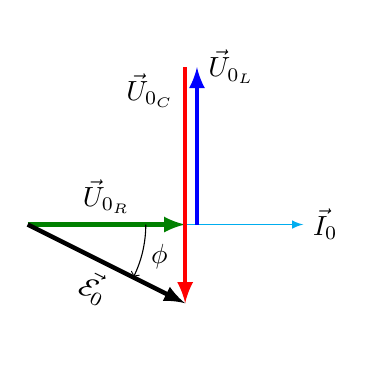
\begin{tikzpicture}[
				declare function = {
						UC = 3;
						UL = 2;
						UR = 2;
						DLC = (UL - UC);
						PhU = atan (DLC/UR);
					},
			]
			\path[use as bounding box] (0,-1.5) rectangle ++(4,4);
			\draw[-latex, cyan] (0,0) -- ++(3.5,0) node[right, color=black] {$\vec{I}_0$};
			\draw[-latex,  green!50!black,ultra thick] (0,0) -- ++(UR,0) node[above, pos=0.5, color=black] {$\vec{U}_{0_R}$};
			\draw[-latex,  blue, ultra thick] (UR+0.15,0) -- ++(0,UL) node[right, color=black] {$\vec{U}_{0_L}$};
			\draw[-latex,  red, ultra thick] (UR,UL) -- ++(0,-UC) node[left, color=black, pos=0.1] {$\vec{U}_{0_C}$};
			\draw[-latex,  black, ultra thick] (0,0) -- (PhU:{UR/cos(PhU)}) node[below, color=black, pos=0.5, sloped] {$\vec{\mathcal{E}}_{0}$} coordinate (U);
			%	\draw[dashed] (\UR,0) -- (U) (0,\DLC) -- (U);
			\draw[->] (0,0) ++(1.5,0) arc(0:PhU:1.5) node[pos=0.6, right] {$\phi$};
		\end{tikzpicture}
		\caption{$\omega < \omega_0$}
		\label{pic:S-vector_diagrams<}
	\end{subfigure}
	\begin{subfigure}[b]{0.30\linewidth}
		\centering
		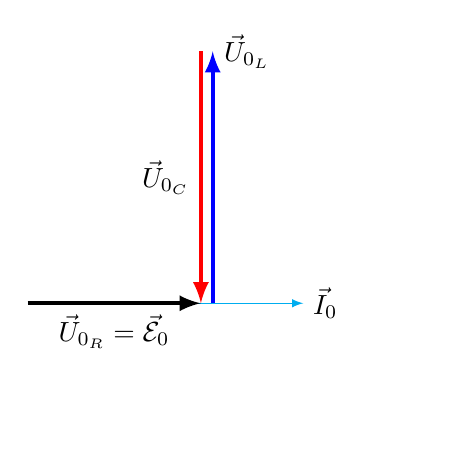
\begin{tikzpicture}[
				declare function = {
						UC = 3.2;
						UL = 3.2;
						UR = 2.2;
						DLC = (UL - UC);
						PhU = atan (DLC/UR);
					},
			]
			\path[use as bounding box] (0,-1.5) rectangle ++(5,5);
			\draw[-latex, cyan] (0,0) -- ++(3.5,0) node[right, color=black] {$\vec{I}_0$};
			\draw[-latex,  black,ultra thick] (0,0) -- ++({2/cos(atan(1/2.2)},0) node[below, pos=0.5, color=black] {$\vec{U}_{0_R} = \vec{\mathcal{E}}_{0}$};
			\draw[-latex,  blue, ultra thick] (UR+0.15,0) -- ++(0,UL) node[right, color=black] {$\vec{U}_{0_L}$};
			\draw[-latex,  red, ultra thick] (UR,UL) -- ++(0,-UC) node[left, color=black, pos=0.5] {$\vec{U}_{0_C}$};
		\end{tikzpicture}
		\caption{$\omega = \omega_0$}
		\label{pic:S-vector_diagrams=}
	\end{subfigure}
	\begin{subfigure}[b]{0.30\linewidth}
		\centering
		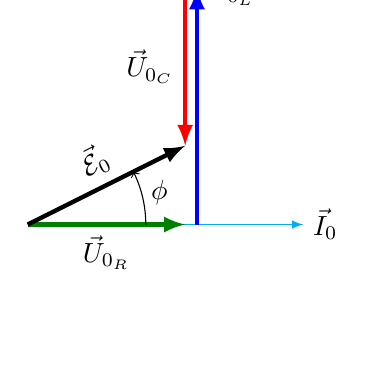
\begin{tikzpicture}[
				declare function = {
						UC = 2;
						UL = 3;
						UR = 2;
						DLC = (UL - UC);
						PhU = atan (DLC/UR);
					},
			]
			\path[use as bounding box] (0,-1.5) rectangle ++(4,4);
			\draw[-latex, cyan] (0,0) -- ++(3.5,0) node[right, color=black] {$\vec{I}_0$};
			\draw[-latex,  green!50!black,ultra thick] (0,0) -- ++(UR,0) node[below, pos=0.5, color=black] {$\vec{U}_{0_R}$};
			\draw[-latex,  blue, ultra thick] (UR+0.15,0) -- ++(0,UL) node[right, color=black] {$\vec{U}_{0_L}$};
			\draw[-latex,  red, ultra thick] (UR,UL) -- ++(0,-UC) node[left, color=black, pos=0.5] {$\vec{U}_{0_C}$};
			\draw[-latex,  black, ultra thick] (0,0) -- (PhU:{UR/cos(PhU)}) node[above, color=black, pos=0.5, sloped] {$\vec{\mathcal{E}}_{0}$} coordinate (U);
			%	\draw[dashed] (\UR,0) -- (U) (0,\DLC) -- (U);
			\draw[->] (0,0) ++(1.5,0) arc(0:PhU:1.5) node[pos=0.6, right] {$\phi$};
		\end{tikzpicture}
		\caption{$\omega > \omega_0$}
		\label{pic:S-vector_diagrams>}
	\end{subfigure}
%	\caption{Векторні діаграми напруг для послідовного кола. \\ {\small \itshape Зсув фаз $\phi$ прийнято позначати стрілкою, яка напрямлена від вектора струму до вектора напруги}}
%	\label{pic:S-vector_diagrams}
%\end{figure}

З формули~\eqref{CI0} видно, що за умови коли частота генератора співпаде з власною частотою контура $\omega = \omega_0 = \frac{1}{\sqrt{LC}}$, реактивні опори котушки і конденсатора стануть однаковими:
\begin{equation}
	\omega L = \frac{1}{\omega C},
\end{equation}
а амплітуда сили струму в послідовному $RLC$-колі досягає свого максимального значення $I_0 = \dfrac{\mathcal{E}_0}{R}$ як і напруга на резисторі, яка дорівнює амплітудному значенню напруги на генераторі $\mathcal{E}_0$. Напруги на конденсаторі і котушці при цьому приймають однакові значення (див. формули~\eqref{U0R} -- \eqref{U0L}):
\begin{align}\label{ULC}
	U_{0_R}    & = \mathcal{E}_0                                                             \\
	U_{0_C}    & = U_{0_L} = \frac{1}{R} \sqrt{\frac{L}{C}} \mathcal{E}_0 = Q \mathcal{E}_0, \label{eq:Q}\\
	U_{0_{LC}} & = U_{0_L} - U_{0_C} = 0 
\end{align}
де $U_{0_{LC}}$~--- амплітуда напруги на $LC$-ділянці. Також слід відмітити, що амплітуди напруги на конденсаторі та котушці індуктивності перевищують напругу на генераторі у $Q$  разів (див.~\eqref{eq:Q}), де

\begin{equation}\label{eq:Qdef}
    Q = \frac{1}{R}\sqrt{\frac{L}{C}}.
\end{equation}
Величина $Q$ називається \href{http://femto.com.ua/articles/part_1/1110.html}{\emph{добротністю контуру}}, її значення завжди більше одиниці (рис.~\ref{plt:S-AFC}). Отже, явище перевищення амплітуд напруг на конденсаторі та котушці в $Q$ разів порівнянні з амплітудою напруги на генераторі в послідовному контурі при співпадінні частоти генератора і власної частоти кола називається \emph{резонансом напруг}. 

%\noindent\bigskip%
%\begin{More}
%
%	З фізичної точки зору, при явищі резонансу напруг в колі відбувається обмін енергією між магнітним полем котушки і електричним полем конденсатора, при такому обміні енергією між полем і джерелом живлення не відбувається.
%\end{More}

\subsection{Енергетичні процеси в послідовному $RLC$-колі}

Фізичний сенс добротності можна побачити, якщо перейти до аналізу енергетичних процесів в коливальному контурі. Розглянемо середню потужність, яка розсіюється контуром у вигляді теплоти за період:
\begin{equation}\label{eq:Power}
    P = \frac12 I_0^2R = \frac12 \frac{\mathcal{E}_0^2R}{R^2 + \left(\omega L - \frac{1}{\omega C}\right)^2} = \frac{\mathcal{E}_0^2}{2R}\, \frac{1}{1  + \left(\omega^2 - \omega_0^2\right)^2 L^2/(R\omega^2)},
\end{equation}
де $I_0$~--- амплітуда коливань струму. Крива, яка описується формулою~\eqref{eq:Power}
 має вигляд, зображений на рис.~\ref{plt:P(o)}.

%---------------------------------------------------------
\begin{center}%[!htbp]\centering
		% !TeX program = lualatex
% !TeX encoding = utf8
% !TeX spellcheck = uk_UA
% !TeX root =../LabWork.tex

		\begin{tikzpicture}
			\pgfset{fpu=true}
			\pgfmathsetmacro{\L}{2e-3}
			\pgfmathsetmacro{\C}{2.2e-6}
			\pgfmathsetmacro{\R}{10}
			\pgfmathsetmacro{\RL}{0.8}
			\pgfmathsetmacro{\Ri}{5}
			\pgfmathsetmacro{\U}{5}
			\pgfmathsetmacro{\omegares}{1/sqrt(\L*\C)}
			\pgfmathsetmacro{\Q}{sqrt(\L/\C)/\RL}
			\pgfmathsetmacro{\Imax}{\U/(\R + \Ri + \RL)}
			\pgfset{fpu=false}
			\begin{axis}[clip = false,
					% === Налаштування сітки ===
					grid = both,
					grid style={line width=.1pt, draw=gray!10},
					major grid style={line width=.2pt,draw=gray!50},
					minor tick num = 5,
					minor grid style = {line width=.1pt,draw=gray!10},
					% === Налаштування положення координатних осей ===
					%axis x line=center, % top, center, bottom
					%axis y line=center, % left, center, right
					axis lines = middle,
					axis line style={-stealth},
					% === Підпис координатних осей ===
					xticklabels={},
					%xlabel={$\omega$},
					ylabel={$\frac{P}{P_{\max}}$},
					xtick scale label code/.code={$\omega$},
					yticklabels={},
					xtick style={draw=none},
					ytick style={draw=none},
					% === Положення підпису координатних осей ===
					%				xlabel style={below right},
					ylabel style={above right},
					every x tick scale label/.style={at={(1,0)}, anchor = north},
					extra y ticks={1/2, 1},
					extra x ticks={\omegares},
					extra y tick labels={$\frac12$, $1$},
					extra x tick labels={$\omega_0$},
					% === Вибір підписів шкали для відображення ===
					xtick = {},
					ytick = {},
					% === Налаштування мінімальних та максимальних значень координат ===
					xmin = 0,
					xmax =  2*\omegares,
					ymin = 0,
					ymax =  1,
					% === Налаштування розміру графіка ===
					width=1\linewidth,
					height=1\linewidth,
				]
				\addplot [ultra thick,samples = 500, green!50!black, thick, domain=0.5*\omegares:2*\omegares, name path global=ResCurve] {(\R + \RL + \Ri)^2/((\R + \RL + \Ri)^2 + (x*\L-1/(\C*x))^2)};

				\path[name path=line] (axis cs:0, {1/2}) -- (axis cs:3*\omegares,{1/2});
				\draw [thick,
					dashed,
					name intersections={of=ResCurve and line},
				] (axis cs:0, {1/2}) -- (intersection-1) -- (intersection-2) (intersection-1) -- (intersection-1 |-0,0) node [below left] {$\omega_0 - \Delta\omega$} (intersection-2) -- (intersection-2 |-0,0) node [below right] {$\omega_0 + \Delta\omega$};
				\fill [white, draw=green!50!black, name intersections={of=ResCurve and line}] (intersection-1) circle (0.1cm) (intersection-2) circle (0.1cm);
			\end{axis}
		\end{tikzpicture}
		\captionof{figure}{Резонансна крива потужності, що розсіюється на резисторі в послідовному контурі}
		\label{plt:P(o)}
\end{center}
%---------------------------------------------------------

При резонансі потужність досягає максимального значення $P_{\max} = \frac12\frac{\mathcal{E}_0^2}{R}$. З фізичної точки зору, це означає, що вся енергія, яка підводиться до кола розсіюється на резисторі, а енергія, яка була запасена в  конденсаторі та котушці індуктивності у вигляді електромагнітного поля, циркулює між цими цими елементами, тобто обмін енергією між полем і джерелом живлення не відбувається.  Ця ситуація виглядає так, ніби зовнішня напруга прикладена лише до резистора. Якщо контур мало поглинає, а більше запасає енергії, то потужність, що розсіюється помітна лише поблизу резонансу на частоті $\omega_0$ і в формул~\eqref{eq:Power} можна скористатись наближенням:
\[
    \omega^2 - \omega_0^2 \approx 2\omega_0\Delta\omega, 
\]
і переписати \eqref{eq:Power} у вигляді:
\begin{equation}\label{eq:Power2}
    P =  \frac{\mathcal{E}_0^2}{2R}\, \frac{1}{1  + (\Delta\omega)^2\tau^2 },
\end{equation}
де $\tau = 2L/R$. З цієї формули видно, що потужність, вдвічі меншу за максимальну можна знайти, якщо  в знаменнику покласти $(\Delta\omega)^2\tau^2 = 1$, тобто коли $\Delta\omega = \frac{R}{2L}$. Величина $\Delta\omega$ називається півшириною резонансної кривої (в радіотехніці вона називається смугою пропускання). Оскільки добротність визначається формулою~\eqref{eq:Qdef}, то легко бачити, що з іншого боку, її можна знайти як
\begin{equation*}
    Q = \frac{1}{R}\sqrt{\frac{L}{C}} = \frac{\omega_0 L}{R} = \frac{\omega_0}{2\Delta\omega},
\end{equation*}
тобто як  відношення резонансної частоти до ширини резонансної кривої потужності. Звідки, зрозуміла назва <<добротність>>, яка означає, що контур тим якісніше (добротніше) чим менше розсіюється в ньому енергії енергії, або чим більше її накопичується за період. Більш високе значення цього показника відповідає більш вузькій кривій, а у випадку ідеального кола ($R = 0$) його добротність нескінченна.

\subsection{Експериментальний метод визначення добротності}

Аналіз резонансної кривої потужності підказує експериментальний спосіб визначення добротності. Ми будемо розглядати в якості резонансної кривої залежність напруги на резисторі як функцію частоти генератора $U_{0R} = f(\omega)$, або  залежність струму в контурі від тієї ж змінної $I = f(\omega)$ (це не суттєво, оскільки ці величини відрізняються лише множником $R$), а ширину кривої $2\Delta\omega$ визначати на $\dfrac1{\sqrt2}\approx 0.707$ від висоти максимуму (рис.~\ref{plt:I(o)}),  оскільки потужність і енергія пропорційні квадрату амплітуди коливань $P \sim I_0^2 \sim U_0^2 $, то рівню $0.707$ відповідає точка половинної потужності, тобто $(0.707)^2 = 0.5$, а добротність також можна визначити за формулою 
\begin{equation*}
Q = \frac{\omega_0}{2\Delta\omega}
\end{equation*}
з урахуванням вищесказаного.

%---------------------------------------------------------
\begin{figure}[!h]\centering
	\begin{minipage}{0.75\linewidth}
		% !TeX program = lualatex
% !TeX encoding = utf8
% !TeX spellcheck = uk_UA
% !TeX root =../LabWork.tex

		\begin{tikzpicture}
			\pgfset{fpu=true}
			\pgfmathsetmacro{\L}{2e-3}
			\pgfmathsetmacro{\C}{2.2e-6}
			\pgfmathsetmacro{\R}{10}
			\pgfmathsetmacro{\RL}{0.8}
			\pgfmathsetmacro{\Ri}{5}
			\pgfmathsetmacro{\U}{5}
			\pgfmathsetmacro{\omegares}{1/sqrt(\L*\C)}
			\pgfmathsetmacro{\Q}{sqrt(\L/\C)/\RL}
			\pgfmathsetmacro{\Imax}{\U/(\R + \Ri + \RL)}
			\pgfset{fpu=false}
			\begin{axis}[clip = false,
					% === Налаштування сітки ===
					grid = both,
					grid style={line width=.1pt, draw=gray!10},
					major grid style={line width=.2pt,draw=gray!50},
					minor tick num = 5,
					minor grid style = {line width=.1pt,draw=gray!10},
					% === Налаштування положення координатних осей ===
					%axis x line=center, % top, center, bottom
					%axis y line=center, % left, center, right
					axis lines = middle,
					axis line style={-stealth},
					% === Підпис координатних осей ===
					xticklabels={},
					%xlabel={$\omega$},
					ylabel={$\frac{I_{0}}{I_{\max}}$},
					xtick scale label code/.code={$\omega$},
					yticklabels={},
					xtick style={draw=none},
					ytick style={draw=none},
					% === Положення підпису координатних осей ===
					%				xlabel style={below right},
					ylabel style={above right},
					every x tick scale label/.style={at={(1,0)}, anchor = north},
					extra y ticks={1/sqrt(2), 1},
					extra x ticks={\omegares},
					extra y tick labels={$\frac{1}{\sqrt2}$, $1$},
					extra x tick labels={$\omega_0$},
					% === Вибір підписів шкали для відображення ===
					xtick = {},
					ytick = {},
					% === Налаштування мінімальних та максимальних значень координат ===
					xmin = 0,
					xmax =  3*\omegares,
					ymin = 0,
					ymax =  1,
					% === Налаштування розміру графіка ===
					width=1\linewidth,
					height=1\linewidth,
				]
				\addplot [ultra thick,samples = 500, green!50!black, thick, domain=0.1*\omegares:3*\omegares, name path global=ResCurve] {(\R + \RL + \Ri)/sqrt((\R + \RL + \Ri)^2 + (x*\L-1/(\C*x))^2)};

				\path[name path=line] (axis cs:0, {1/sqrt(2)}) -- (axis cs:3*\omegares,{1/sqrt(2)});
				\draw [thick,
					dashed,
					name intersections={of=ResCurve and line},
				] (axis cs:0, {1/sqrt(2)}) -- (intersection-1) -- (intersection-2) (intersection-1) -- (intersection-1 |-0,0) node [below left] {$\omega_0 - \Delta\omega$} (intersection-2) -- (intersection-2 |-0,0) node [below right] {$\omega_0 + \Delta\omega$};
				\fill [white, draw=green!50!black, name intersections={of=ResCurve and line}] (intersection-1) circle (0.1cm) (intersection-2) circle (0.1cm);
			\end{axis}
		\end{tikzpicture}
		\caption{Амплітудно-частотна характеристика напруги на резисторі послідовного контуру}
		\label{plt:I(o)}
	\end{minipage}
\end{figure}
%---------------------------------------------------------

Розглянемо тепер, як поводить себе модуль імпедансу всього контура, та модуль імпедансу $LC$-ділянки (рис.~\ref{plt:impedance_character}). З графіків видно, що за умови, коли частота генератора менше частоти резонансної частоти кола, ємнісний опір переважає над індуктивним і контур представляє для генератора опір ємнісного характеру. Якщо частота генератора більше резонансної частоти кола, то індуктивний опір більше ємнісного і контур для генератора є опором індуктивного характеру. При резонансі опір кола є суто активним.

%---------------------------------------------------------
\begin{figure}[!h]\centering
	% !TeX program = lualatex
% !TeX encoding = utf8
% !TeX spellcheck = uk_UA
% !TeX root =../LabWork.tex

	\begin{tikzpicture}[
			declare function={
					L  = 2;
					C  = 1.2e-3;
					R  = 80;
					omegares  = 1/sqrt(L*C);
					Q  = sqrt(L/C)/R;
					XL(\x) =\x*L;
					XC(\x) = 1/(C*\x) ;
				},
		]
		\begin{axis}[
				% === Налаштування сітки ===
				grid = both,
				major grid style={line width=.2pt,draw=gray!50},
				minor tick num = 4,
				minor grid style = {line width=.1pt,draw=gray!10},
				extra tick style={% changes for all extra ticks
						tick align=outside,
						grid style={dashed,draw=black}
					},
				extra x tick style={
						tick label style={
								xshift=5mm,
								/pgf/number format/.cd, fixed, fixed zerofill,
							}
					},
				% === Налаштування положення координатних осей ===
				axis lines = middle,
				axis line style={stealth-stealth},
				% === Підпис коор5динатних осей ===
				%				xticklabels={},
				xlabel={$\omega$},
				ylabel={},
				% === Положення підпису координатних осей ===
				ylabel style={above right},
				xticklabels={},
				yticklabels={},
				extra x ticks = {omegares},
				extra x tick labels = {$\omega_0$},
				ytick style={draw=none},
				xtick style={draw=none},
				% === Вибір підписів шкали для відображення ===
				xtick = {},
				ytick = {},
				legend style={at={(current axis.south east)},anchor=south east},
				% === Налаштування мінімальних та максимальних значень координат ===
				xmin = 6,
				xmax =  60,
				ymin = -150,
				ymax =  150,
				% === Налаштування розміру графіка ===
				width=1\linewidth,
				width=0.7\linewidth,
			]
			\addplot [ultra thick,samples = 500, blue, thick, domain=0.2*omegares:3*omegares,name path = UL]  {XL(x)};
			\addplot [ultra thick,samples = 500, red, thick, domain=0.2*omegares:3*omegares,name path = UC]  {-XC(x)};
			\addplot [ultra thick,samples = 500, green!50!black, thick, domain=0.2*omegares:3*omegares,name path = DU]  {XL(x)-XC(x)};
			\addplot [ultra thick,samples = 500, black, thick, domain=0.2*omegares:3*omegares,name path = DU]  {sqrt(R^2 + (XL(x)-XC(x))^2)};
			\legend{$X_L = \omega L$, $X_C = \frac{1}{\omega C}$, $Z_{LC} = X_L - X_C$, $Z = \sqrt{R^2 + (X_L - X_C)^2}$}
			\pgfplotsinvokeforeach{0.5,1,2}{
				\draw [-latex, blue, ultra thick] (axis cs:#1*omegares, 0) -- node[left] {$X_L$} (axis cs:#1*omegares, {XL(#1*omegares)});
				\draw [-latex, red, ultra thick] (axis cs:#1*omegares, 0) -- node[left] {$X_C$} (axis cs:#1*omegares, {-XC(#1*omegares)});
			}
			\draw [latex-latex, black] (axis cs:0.6*omegares, 0) -- node[fill=white] {$R$} (axis cs:0.6*omegares, {R});
			\draw [dashed] (axis cs:omegares, R) -- (axis cs:0.6*omegares, R);
		\end{axis}
	\end{tikzpicture}
	\caption{Характер зміни імпедансу кола}
	\label{plt:impedance_character}
\end{figure}

\noindent\bigskip%
\begin{More}

    В електротехніці резонанс напруг є небажаним явищем, оскільки він викликає перенапруження і вихід з ладу обладнання. Як простий приклад можна привести довгу кабельну лінію, яка з якоїсь причини виявилася не підключеною до навантаження, але при цьому живиться від проміжного трансформатора. Така лінія з розподіленою ємністю і індуктивністю, якщо її резонансна частота співпаде з частотою мережі живлення, просто буде пробита і вийде з ладу.

	Явище резонансу напруг використовують в \emph{електричних фільтрах}, наприклад якщо необхідно усунути з сигналу, що передається, складову струму певної частоти, то паралельно приймачу ставлять ланцюжок із сполучених послідовно конденсатора і котушки індуктивності, щоб струм резонансної частоти цього $LC$-ланцюжка замкнулося б через нього, і не потрапив до приймача. Тоді струми частоти далекою від резонансної частоти $LC$-ланцюжка будуть проходити в навантаження безперешкодно, і тільки близькі до резонансу по частоті струми --- знаходитимуть собі найкоротший шлях через $LC$-ланцюжок.

	Резонанс напруг широко застосовують в радіотехніці і використовують в тих випадках, коли потрібно посилити коливання напруги будь-якої визначеної частоти, при настроюванні радіоприймача на потрібну довжину хвилі. Вибірність приймача буде тим більшою, чим <<гостріша>> резонансна крива струму. Але уява про те, що під час радіоприймання потрібно, по можливості, збільшувати добротність контуру, бо при цьому збільшується напруга на конденсаторі, тобто чутливість приймача і усувається вплив сусідніх станцій, оскільки резонансна крива звужується, є помилкова, оскільки сигнал ніколи не буває ідеально монохроматичним. Тому, якщо крива резонансу надзвичайно вузька, то частина спектральних складових сигналу опиниться поза смугою пропускання контуру, що призведе до викривлення сигналу. Тому, наприклад, в телебаченні при передачі сигналів зображення використовується широка смуга частот 

\end{More}

\section{Резонанс струмів у паралельному $RLC$-колі}

Розглянемо електричне коло, де котушка, конденсатор та резистор з'єднані паралельно (рис.~\ref{pic:P-RLC}). В цьому випадку, напруга на кожному елементі буде однакова, а загальний струм $I$ буде дорівнювати сумі струмів, що протікають через кожний з елементів:
\begin{equation}
	I = I_R + I_C +I_L.
\end{equation}

В цьому випадку також можна скористатись методом комплексних амплітуд і визначити струми на окремих елементах контуру та загальний струм в колі:

\begin{align}
	I_R & = \frac{\mathcal{E}_0}{R} \cos(\omega t), \label{IR}                                                                     \\
	I_C & = \mathcal{E}_0\omega C \cos (\omega t + \frac{\pi}{2}), \label{IC}                                                      \\
	I_L & = \frac{\mathcal{E}_0}{\omega L}\cos (\omega t - \frac{\pi}{2}), \label{IL}                                              \\
	I   & = \mathcal{E}_0\sqrt{\frac{1}{R^2}  +   \left(  \omega C - \frac{1}{\omega L} \right)^2} \cos(\omega t + \phi).\label{I}
\end{align}

Зсув фаз $\phi$ між напругою та загальним струмом у колі дорівнюватиме:
\begin{equation}\label{P-phase_shift}
	\tg\phi = \frac{\omega C - \frac{1}{\omega L}}{R}.
\end{equation}

\begin{wrapfigure}[]{L}{0.4\linewidth}
	\begin{tikzpicture}[every circuit symbol/.style={thick}]
		\draw[thick] (0,-2) coordinate (START) to [ac source={rotate=-90,info={left:$\mathcal{E}_0$}}] (0,2) coordinate (AC) -- ++(2,0) coordinate (A) to [resistor={info'={$R$}}] ++(0,-4) coordinate (B) -- (START)
		(A) -- ++(1.5,0) coordinate (A1) to [capacitor={info'={$C$}}] ++(0,-4) coordinate (B1) -- (B)
		(A1) -- ++(1.5,0) coordinate (A2) to [inductor={info'={$L$}}] ++(0,-4) -- (B1)
		;
		\draw[->,red, thick] ([xshift=0.25cm]AC) -- node[color=black, above] {$I$} ++(1,0);
		\draw[->,red, thick] ([yshift=-0.25cm]A) -- node[color=black, left] {$I_R$} ++(0,-1);
		\draw[->,red, thick] ([yshift=-0.25cm]A1) -- node[color=black, left] {$I_C$} ++(0,-1);
		\draw[<-,red, thick] ([yshift=-0.25cm]A2) -- node[color=black, left] {$I_L$} ++(0,-1);
	\end{tikzpicture}
	\caption{Паралельне $RLC$-коло}
	\label{pic:P-RLC}
\end{wrapfigure}
З цих формул видно, що струм на резисторі $I_R$ коливається в фазі з напругою на генераторі, а його амплітуда не залежить від частоти, крім того, струми на конденсаторі $I_C$ і котушці $I_L$ коливаються в протифазі, і їх амплітуди залежать від частоти.

При частоті $\omega_0 = \dfrac{1}{\sqrt{CL}}$ амплітуда струму в колі досягає \emph{мінімального} значення $I_{0_{\min}} = I_{0_R}  = \dfrac{\mathcal{E}_0}{R}$, яка називається \emph{резонансною частотою}. При цьому струми на котушці та конденсаторі приймають однакові амплітудні значення $I_{0_C} = I_{0_L} = Q I_{0_{\min}}$, тобто перевищують силу струму в нерозгалудженій ділянці кола в $Q$ разів, при цьому контур поводить себе як активний опір ($\phi = 0$) величиною $Z = RQ^2$. Таке явище називається \emph{резонансом струмів} (рис.~\ref{plt:I(o)}).

%---------------------------------------------------------
\begin{figure}[!h]\centering
	% !TeX program = lualatex
% !TeX encoding = utf8
% !TeX spellcheck = uk_UA
% !TeX root =../LabWork.tex

	\begin{minipage}{0.75\linewidth}
		\begin{tikzpicture}[
			declare function = {
					L  = 2;
					C  = 0.5;
					R  = 10;
					RL  = 0.1;
					U = 2;
					omegares  = 1/sqrt(L*C);
					Q  = sqrt(L/C)/R;
					I(\x) = U*sqrt( (1/R + RL/(RL^2+\x^2*L^2))^2 + (\x*C-L*\x/(RL^2 + L^2*\x^2))^2 );				
				}
			]
			%---------------------------------------------------------
			\begin{groupplot}[group style={group size=1 by 2, vertical sep=2cm}]
				%---------------------------------------------------------
				\nextgroupplot[title={\small Амплітудно-частотна характеристика паралельного кола},
					% === Налаштування сітки ===
					grid = both,
					grid style={line width=.1pt, draw=gray!10},
					major grid style={line width=.2pt,draw=gray!50},
					minor tick num = 5,
					minor grid style = {line width=.1pt,draw=gray!10},
					% === Налаштування положення координатних осей ===
					%axis x line=center, % top, center, bottom
					%axis y line=center, % left, center, right
					axis lines = middle,
					axis line style={-stealth},
					% === Підпис координатних осей ===
					xlabel={$\omega$},
					ylabel={$I$},
					xticklabels={},yticklabels={},
					xtick style={draw=none},
					ytick style={draw=none},
					extra tick style={% changes for all extra ticks
							tick align=outside,
							major grid style={dashed,draw=black}
						},
					extra x ticks = {omegares},
					extra x tick labels={$\omega_0$},
					extra y ticks = {I(omegares),U*omegares*C},
					extra y tick labels={$I_0$, $I_0/Q$},
					% === Положення підпису координатних осей ===
					xlabel style={below right},
					ylabel style={above left},
					% === Вибір підписів шкали для відображення ===
					xtick = {},
					ytick = {},
					% === Налаштування мінімальних та максимальних значень координат ===
					xmin = 0,
					xmax =  2,
					ymin = 0,
					ymax =  4,
					% === Налаштування розміру графіка ===
					width=1\linewidth,
					height=0.96\linewidth,
				]
				\addplot [ultra thick,samples = 500, green!50!black, thick,domain=0:2, restrict y to domain=0:4, name path global=ResCurve] {I(x)};
				\addplot [ultra thick,samples = 500, red, thick, domain=0:2, restrict y to domain=0:4] {U*x*C};
				\addplot [ultra thick,samples = 500, blue, thick, domain=0:2, restrict y to domain=0:4] {U/sqrt(x^2*L^2 + RL^2)};
				\legend{$I_0$, $I_{0_C}$, $I_{0_L}$}
				%---------------------------------------------------------
				\nextgroupplot[title={\small Фазово-частотна характеристика паралельного кола},
					% === Налаштування сітки ===
					grid = both,
					grid style={line width=.1pt, draw=gray!10},
					major grid style={line width=.2pt,draw=gray!50},
					minor tick num = 4,
					minor grid style = {line width=.1pt,draw=gray!10},
					% === Налаштування положення координатних осей ===
					axis lines = middle,
					yticklabel pos=right,
					axis line style={-stealth},
					% === Підпис координатних осей ===
					xlabel={$\omega$},
					ylabel={$\phi$},
					xticklabels={},
					yticklabels={},
					extra tick style={% changes for all extra ticks
							tick align=outside,
							grid style={dashed,draw=black}
						},
%					extra y tick style={
%	
%						},
					extra x ticks = {omegares},
					extra x tick labels={$\omega_0$},
					extra y ticks = {-pi/2,pi/2},
					ytick = {-pi/2,-pi/4,0,pi/4,pi/2},
					extra y tick labels={$-\frac{\pi}{2}$,$\frac{\pi}{2}$},
					xtick style={draw=none},
					ytick style={draw=none},
					% === Положення підпису координатних осей ===
					xlabel style={below right},
					ylabel style={above right},
					% === Налаштування мінімальних та максимальних значень координат ===
					xmin = 0,
					xmax =  2*omegares,
					ymin = -pi/2,
					ymax =  pi/2,
					% === Налаштування розміру графіка ===
					width=1\linewidth,
					height=0.4\linewidth,
				]
				\addplot [ultra thick,samples = 1000, green!50!black, thick, domain=0.01:2*omegares, name path global=ResCurve] {rad(-atan((x*L-1/(x*C))/RL))};
				%---------------------------------------------------------
			\end{groupplot}
		\end{tikzpicture}
	\caption{Амплітудно- і фазовочастотні характеристики паралельного кола}
	\label{plt:P-AFC}
	\end{minipage}
\end{figure}
%---------------------------------------------------------

%\begin{figure}[h!]\centering
%            % !TeX program = lualatex
% !TeX encoding = utf8
% !TeX spellcheck = uk_UA
% !TeX root =../LabWork.tex

	\begin{subfigure}[b]{0.30\linewidth}
		\centering
		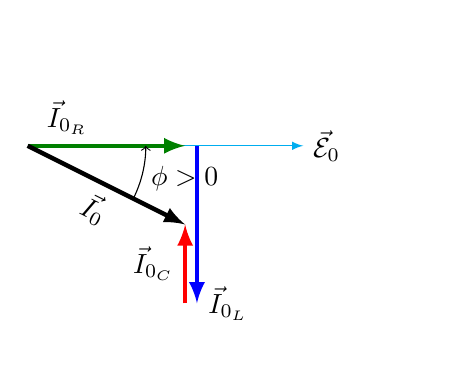
\begin{tikzpicture}[
				declare function = {
						IC = 1;
						IL = 2;
						IR = 2;
						DLC = (IL - IC);
						PhI = -atan(DLC/IR);
					},
			]
			\path[use as bounding box] (0,1.5) rectangle ++(5,-4);
			\draw[-latex, cyan] (0,0) -- ++(3.5,0) node[right, color=black] {$\vec{\mathcal{E}}_0$};
			\draw[-latex,  green!50!black,ultra thick] (0,0) -- ++(IR,0) node[above, pos=0.25, color=black] {$\vec{I}_{0_R}$};
			\draw[-latex,  blue, ultra thick] (IR+0.15,0) -- ++(0,-IL) node[right, color=black] {$\vec{I}_{0_L}$};
			\draw[-latex,  red, ultra thick] (IR,-IL) -- ++(0,IC) node[left, color=black, pos=0.5] {$\vec{I}_{0_C}$};
			\draw[-latex,  black, ultra thick] (0,0) -- (PhI:{IR/cos(PhI)}) node[below, color=black, pos=0.5, sloped] {$\vec{I}_{0}$} coordinate (I);
			\draw[<-] (0,0) ++(1.5,0) arc(0:PhI:1.5) node[pos=0.6, right] {$\phi > 0$};
		\end{tikzpicture}
		\caption{$\omega < \omega_0$}
		\label{pic:P-vector_diagrams<}
	\end{subfigure}
	\begin{subfigure}[b]{0.30\linewidth}
		\centering
		\begin{tikzpicture}[
				declare function = {
						IC = 1.5;
						IL = 1.5;
						IR = 2;
						DLC = (IL - IC);
						PhI = -atan(DLC/IR);
					},
			]
			\path[use as bounding box] (0,1.5) rectangle ++(5,-4);
			\draw[-latex, cyan] (0,0) -- ++(3.5,0) node[right, color=black] {$\vec{\mathcal{E}}_0$};
			\draw[-latex,  green!50!black,ultra thick] (0,0) -- ++(IR,0) node[above, pos=0.5, color=black] {$\vec{I}_{0_R} = \vec{I}_{0}$};
			\draw[-latex,  blue, ultra thick] (IR+0.15,0) -- ++(0,-IL) node[right, color=black] {$\vec{I}_{0_L}$};
			\draw[-latex,  red, ultra thick] (IR,-IL) -- ++(0,IC) node[left, color=black, pos=0.2] {$\vec{I}_{0_C}$};
		\end{tikzpicture}
		\caption{$\omega = \omega_0$}
		\label{pic:P-vector_diagrams=}
	\end{subfigure}
	\begin{subfigure}[b]{0.30\linewidth}
		\centering
		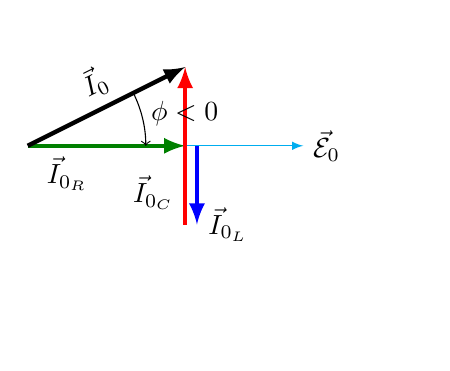
\begin{tikzpicture}[
				declare function = {
						IC = 2;
						IL = 1;
						IR = 2;
						DLC = (IL - IC);
						PhI = -atan(DLC/IR);
					},
			]
			\path[use as bounding box] (0,1.5) rectangle ++(5,-4);
			\draw[-latex, cyan] (0,0) -- ++(3.5,0) node[right, color=black] {$\vec{\mathcal{E}}_0$};
			\draw[-latex,  green!50!black,ultra thick] (0,0) -- ++(IR,0) node[below, pos=0.25, color=black] {$\vec{I}_{0_R}$};
			\draw[-latex,  blue, ultra thick] (IR+0.15,0) -- ++(0,-IL) node[right, color=black] {$\vec{I}_{0_L}$};
			\draw[-latex,  red, ultra thick] (IR,-IL) -- ++(0,IC) node[left, color=black, pos=0.2] {$\vec{I}_{0_C}$};
			\draw[-latex,  black, ultra thick] (0,0) -- (PhI:{IR/cos(PhI)}) node[above, color=black, pos=0.5, sloped] {$\vec{I}_{0}$} coordinate (I);
			\draw[<-] (0,0) ++(1.5,0) arc(0:PhI:1.5) node[pos=0.6, right] {$\phi < 0$};
		\end{tikzpicture}
		\caption{$\omega > \omega_0$}
		\label{pic:P-vector_diagrams>}
	\end{subfigure}
%	\caption{Векторні діаграми струмів для паралельного кола}
%	\label{pic:P-vector_diagrams}
%\end{figure}
%---------------------------------------------------------

При виникненні резонансу струму в колі його  реактивна складова стає рівною нулю, і як наслідок, повна провідність кола знижується до мінімального значення. Тому при постійній напрузі на затискачах даної схеми струм в нерозгалудженій частині  стає мінімальний, на відміну від резонансу напруги, коли струм максимальний. При цьому сумарний струм даному колі буде дорівнює векторній сумі всіх трьох струмів, два з яких (а саме $I_L$ і $I_C$) знаходяться в протифазі. Саме із-за того, що $I_L$ і $I_C$ знаходяться в протифазі в $LC$-ділянці починає протікати струм, який при резонансі може значно перевищувати сумарний струм $I$.

\noindent\bigskip%
\begin{More}

	Явище резонансу струмів використовується в прийомних пристроях для виділення електромагнітного сигналу в вузькому спектральному інтервалі частот поблизу резонансної частоти.

	В індукційних печах паралельно котушці, що створює змінне магнітне поле, підключають ємність. Якщо умови резонансу виконуються, то струм в котушці збільшується в багато разів, а струм в підвідних проводах при цьому відносно невеликий.
\end{More}


